\begin{abstract}
	Les deux approches basées sur les algorithmes génétiques présentées en chapitre \ref{chap:materiel_et_solutions} sont testées. Il en ressort que sur les instances proposées par Houndji \cite{houndji_thesis}, les deux approches parviennent à trouver des solutions très proches des solutions optimales assez rapidement. Elles ne parviennent cependant pas à en faire autant sur les grandes instances proposées par Ceschia \cite{ceschia}.
\end{abstract}

\section*{Introduction}
		\addcontentsline{toc}{section}{Introduction}
		Dans ce chapitre, nous testons les théories émises et analysons les résultats obtenus de tests afin de vérifier nos approches de solution du problème énoncées. A cette fin, nous présentons d'abord les données (instances) et paramètres de test. Ensuite, nous expérimentons nos solutions et à partir des résultats obtenus, nous comparons nos approches heuristiques basées sur les algorithmes génétiques à celles déjà appliquées à ce problème.
		
\section{Données et paramètres de test}
	\subsection*{Données de test}
Afin de tester nos deux solutions, nous commençons dans un premier temps par utiliser un ensemble de 20 instances des 100 proposées par Houndji et al. \cite{houndji_thesis} auxquelles ils ont appliqué la CP. Ces instances sont caractérisées par un nombre de périodes \emph{NT} = 20 , un nombre d'articles \emph{NI} = 5 et un nombre de demandes \emph{ND} = 20. Le choix de ces 20 instances s'est fait de la manière suivante: nous avons choisi les 5 premières instances des 100 proposées par Houndji, puis nous avons ensuite choisi 15 autres en veillant à combiner les instances sur lesquelles l'approche CP prenait le plus de temps et celles où elle en prenait le moins. Les résultats seront comparés à ceux obtenus par Houndji et al. dans leur application de l'approche CP à ces instances. \\
		\hspace*{.5cm} Dans un second temps, nous appliquons nos deux solutions à 6 autres instances des 27 proposées par Ceschia et al \cite{ceschia} dans leur bibliothèque Opthub. En effet, dans le but de tester leur approche de solution basée sur le recuit simulé aux instances de PSP, Ceschia et al (au même titre que Houndji dans son expérimentation du CP) ont  développé un générateur paramétré produisant de nouvelles instances plus grandes. Le générateur travaille de sorte que l'instance produite est faisable, c'est à dire qu'elle satisfait aux contraintes de \emph{NoBacklog}. Nous testons notre approche de solution sur ces nouvelles grandes instances et comparons nos résultats à ceux obtenus par Ceschia et al dans leur application du recuit simulé à ces instances. \\
		\hspace*{.5cm} Dans les deux cas, nos critères d'analyse sont de deux ordres. Premièrement, nous avons analysé les résultats sous l'angle de la performance en temps. Il s'agit de voir comment ces algorithmes arrivent à répondre aussi rapidement que possible nos instances de PSP.  Le second angle d'analyse s'est porté sur la performance en terme de la qualité de la solution trouvée. Nous avons calculé l'écart entre la solution trouvée et la solution optimale connue dans la littérature.
		
		\subsection*{Paramètres de test}
		Les paramètres de test utilisés afin d'effectuer les tests sont présentés comme suit selon que le programme implémente \emph{Hierarchical Coarse-grained and Master-slave Parallel Genetic Algorithm} (HCM-PGA) ou \emph{Hierarchical Fine-grained and Coarse-grained Parallel Genetic Algorithm}(HFC-PGA):

		\begin{enumerate}
			\item HCM-PGA \\
				\begin{itemize}
					\item[-] Taille de la population : 25 individus par processus ;
			        \item[-] Probabilité de mutation : 5\%;
			        \item[-] Probabilité de croisement : 80\%;
			        \item[-] Nombre de migrants : 1 individu;
		 	        \item[-] Nombre de processus esclaves : 2 processus;
			        \item[-] Nombre de processus principaux : 2 processus;
			        \item[-] Nombre de générations avant migration : 0 génération (la migration intervient après une convergence).
				\end{itemize}
				\vspace*{.5cm}
			\item HFC-PGA \\
				\begin{itemize}
					\item[-] Taille de la population : 25 individus par processus ;
			        \item[-] Probabilité de mutation : 5\%;
			        \item[-] Probabilité de croisement : 80\%;
			        \item[-] Nombre de migrants : 1 individu;
			        \item[-] Nombre de processus principaux : 2 processus;
			        \item[-] Nombre de générations avant migration : 0 génération (la migration intervient après une convergence).
				\end{itemize}
		\end{enumerate}
		Ces paramètres de test, retenus expérimentalement, sont les valeurs qui nous sont parues maximisant la qualité des solutions trouvées par chacun des algorithmes.		
		
		\section{Résultats expérimentaux des algorithmes génétiques parallèles hiérarchiques \emph{fine-grained} et \emph{coarse-grained}}
		Nous avons testé les algorithmes génétiques parallèles hiérarchiques "fine-grained" et "coarse-grained" dans un premier temps sur 20 instances de PSP proposées par Houndji et dans un second temps sur 6 autres instances de PSP plus grandes proposées par Ceschia. Les résultats de ces tests sont consignés dans les tableaux \ref{tab:hfc_pga_cp} et \ref{tab:hfc_pga_sa}.Ces tables présentent les résultats respectivement de l'approche CP et de l'approche de recuit simulé. Ces tableaux présentent les performances en temps et qualité des solutions des algorithmes génétiques parallèles hiérarchiques "fine-grained" et "coarse-grained". Nous avons effectué nos tests à travers 10 essais sur chacune des instances et obtenu des résultats compilés, une moyenne des performances de notre méthode de résolution proposée.
		
	\begin{table}[h]
		\centering
		\begin{tabular}{|c|c|c|c|c|c|c|}
			\hline
			\textbf{Instance} & \textbf{Opt cost \footnote{Coût de la solution optimale}} & \textbf{CP time \footnote{Temps en secondes de l'approche CP}} & \textbf{GAs time \footnote{Temps moyen en secondes de notre approche génétique}} & \textbf{GAs result gap \footnote{Différence entre la solution optimale et la solution trouvée par notre approche génétique}} & \textbf{GAs Best Sol \footnote{Meilleure solution trouvée par notre approche génétique}} & \textbf{Nb Gen \footnote{Nombre de générations parcourues par notre approche génétique}}\\
			\hline
			\textbf{instance 1} & 1377 & 9.14 & 3.9 & 0.2\% & 1378 & 15 \\
			\textbf{instance 2} & 1447 & 7.292 & 1.7 & 1.67\% & 1447 & 12.8\\
			\textbf{instance 3} & 1107 & 2.946 & 3.2 & 0.07\% & 1108 & 20.2\\
			\textbf{instance 4} & 1182 & 1.784 & 2.4 & 1.4\% & 1199 & 17\\
			\textbf{instance 5} & 1471 & 0.235 & 4.5 & 0\% & 1471 & 17.8\\
			\textbf{instance 8} & 3117 & 25.352 & 10.3 & 0.25\% & 3117 & 15.4\\
			\textbf{instance 21} & 2774 & 11.177 & 2.2 & 0\% & 2774 & 16.3\\
			\textbf{instance 23} & 1473 & 15.039 & 6.1 & 0\% & 1473 & 13\\
			\textbf{instance 35} & 2655 & 12.846 & 2.5 & 0.5\% & 2670 & 16.4\\
			\textbf{instance 36} & 1493 & 121.909 & 6.5 & 0\% & 1493 & 18.3\\
			\textbf{instance 53} & 1108 & 0.935 & 2.6 & 1.8\% & 1128 & 16.7\\
			\textbf{instance 58} & 1384 & 2.347 & 2.11 & 1.9\% & 1411 & 14.2\\
			\textbf{instance 61} & 977 & 0.711 & 2.1 & 0\% & 977 & 14.4\\
			\textbf{instance 69} & 1619 & 1.223 & 2.5 & 0\% & 1619 & 13.1\\
			\textbf{instance 73} & 1104 & 12.508 & 3.8 & 3.7\% & 1145 & 65.6\\
			\textbf{instance 78} & 1297 & 16.187 & 3.04 & 1.3\% & 1297 & 17.9\\
			\textbf{instance 85} & 2113 & 9.404 & 2.47 & 2.3\% & 2162 & 14\\
			\textbf{instance 87} & 1152 & 1.589 & 3.5 & 2.1\% & 1152 & 15.9\\
			\textbf{instance 90} & 2449 & 23.811 & 3.7 & 3.3\% & 2531 & 14.1\\
			\textbf{instance 94} & 1403 & 11.726 & 5.9 & 1.3\% & 1403 & 16\\
			
			\hline
		\end{tabular}	
		\caption{Performances du HFC-PGA et CP sur 20 instances du PSP}	
		\label{tab:hfc_pga_cp}
	\end{table}			
	
	\begin{table}[h]
		\centering
		\begin{tabular}{|c|c|c|c|c|c|c|}
			\hline
			\textbf{Instance} & \textbf{Opt cost} & \textbf{SA time} & \textbf{GAs time} & \textbf{GAs result gap} & \textbf{GAs Best Sol} & \textbf{Nb Gen}\\
			\hline
			\textbf{ps-200-10-80} & 18089 & 72.2 & 9.9 & 8.7\% & 19484 & 18.2 \\
			\textbf{ps-200-20-80} & 19190 & 73.8 & 18.8 & 11.6\% & 21302 & 18.9 \\
			\textbf{ps-300-10-80} & 26343 & 78.4 & 56.8 & 16.5\% & 30452 & 17.3 \\
			\textbf{ps-300-20-80} & 30206 & 68.3 & 96.8 & 7.4\% & 32289 & 20 \\
			\textbf{ps-400-10-80} & 34206 & 85.5 & 117.9 & 19.5\% & 40775 & 25.9 \\
			\textbf{ps-400-20-80} & 41329 & 69.5 & 120.3 & 10.1\% & 45521 & 22.9 \\
			\hline
		\end{tabular}	
		\caption{Performances du HFC-PGA et SA sur 6 instances du PSP}
		\label{tab:hfc_pga_sa}	
	\end{table}			
		
		\section{Résultats expérimentaux des algorithmes génétiques parallèles hiérarchiques \emph{coarse-grained} et \emph{master-slave}}
		
		Après les tests de l'algorithme génétique parallèle hiérarchique \emph{fine-grained} et \emph{coarse-grained}, nous avons procédé aux tests sur l'algorithme génétique parallèle hiérarchique \emph{master-slave} et \emph{coarse-grained} sur les mêmes instances que celles testées ci-dessus. Au bout de 10 essais, les résultats et la moyenne obtenue des essais effectués sont consignés dans les tableaux \ref{tab:hcm_pga_cp}  et \ref{tab:hcm_pga_sa}; et sont comparés respectivement à ceux obtenus en programmation par contrainte et en recuit simulé.
		
		\begin{table}[h]
		\centering
		\begin{tabular}{|c|c|c|c|c|c|c|}
			\hline
			\textbf{Instance} & \textbf{Opt cost} & \textbf{CP time} & \textbf{GAs time} & \textbf{GAs result gap} & \textbf{GAs Best Sol} & \textbf{Nb Gen}\\
			\hline
			\textbf{instance 1} & 1377 & 9.14 & 1.73 & 0.07\% & 1378 & 19.2 \\
			\textbf{instance2} & 1447 & 7.292 & 1.4 & 0.2\% & 1447 & 21.3\\
			\textbf{instance 3} & 1107 & 2.946 & 1.6 & 0\% & 1107 & 17.1\\
			\textbf{instance 4} & 1182 & 1.784 & 1.3 & 1.1\% & 1196 & 21.1\\
			\textbf{instance 5} & 1471 & 0.235 & 2.4 & 8\% & 1601 & 16.5\\
			\textbf{instance 8} & 3117 & 25.352 & 4.08 & 0\% & 3117 & 18.9\\
			\textbf{instance 21} & 2774 & 11.177 & 2.6 & 0\% & 2774 & 18.3\\
			\textbf{instance 23} & 1473 & 15.039 & 1.9 & 0\% & 1473 & 20\\
			\textbf{instance 35} & 2655 & 12.846 & 2.6 & 0.2\% & 2655 & 26\\
			\textbf{instance 36} & 1493 & 121.909 & 3.4 & 0\% & 1502 & 20.5\\
			\textbf{instance 53} & 1108 & 0.935 & 1.5 & 0\% & 1108 & 21.4\\
			\textbf{instance 58} & 1384 & 2.347 & 1.8 & 1.01\% & 1398 & 20.3\\
			\textbf{instance 61} & 977 & 0.711 & 1.6 & 0\% & 977 & 24.1\\
			\textbf{instance 69} & 1619 & 1.223 & 1.7 & 0.9\% & 1635 & 21.5\\
			\textbf{instance 73} & 1104 & 12.508 & 1.8 & 0\% & 1104 & 21.9\\
			\textbf{instance 78} & 1297 & 16.187 & 1.8 & 0.4\% & 1297 & 20.7\\
			\textbf{instance 85} & 2113 & 9.404 & 2.3 & 0.9\% & 2127 & 21.5\\
			\textbf{instance 87} & 1152 & 1.589 & 1.8 & 1.6\% & 1152 & 25\\
			\textbf{instance 90} & 2449 & 23.811 & 2.32 & 2.6\% & 2503 & 24.5\\
			\textbf{instance 94} & 1403 & 11.726 & 2.5 & 0\% & 1403 & 19.7\\
			\hline
		\end{tabular}	
		\caption{Performances du HCM-PGA et CP sur 20 instances du PSP}	
		\label{tab:hcm_pga_cp}	
	\end{table}	
	
	\begin{table}[h]
		\centering
		\begin{tabular}{|c|c|c|c|c|c|c|}
			\hline
			\textbf{Instance} & \textbf{Opt cost} & \textbf{SA time} & \textbf{GAs time} & \textbf{GAs result gap} & \textbf{GAs Best Sol} & \textbf{Nb Gen}\\
			\hline
			\textbf{ps-200-10-80} & 18089 & 72.2 & 11.2 & 10\% & 19799 & 24.4 \\
			\textbf{ps-200-20-80} & 19190 & 73.8 & 11.5 & 11.2\% & 21345 & 18.2 \\
			\textbf{ps-300-10-80} & 26343 & 78.4 & 32.2 & 33\% & 34985 & 20.7 \\
			\textbf{ps-300-20-80} & 30206 & 68.3 & 30.8 & 7\% & 32207 & 22.2 \\
			\textbf{ps-400-10-80} & 34206 & 85.5 & 37.8 & 18.4\% & 40433 & 23.9 \\
			\textbf{ps-400-20-80} & 41329 & 69.5 & 60.9 & 10.3\% & 45647 & 22.9 \\
			\hline
		\end{tabular}	
		\caption{Performances du HCM-PGA et SA sur 6 instances du PSP}	
		\label{tab:hcm_pga_sa}	
	\end{table}					
	
		\section{Discussion}
		Nous effectuons dans cette section une analyse comparative des résultats afin de dégager des conclusions. Ainsi, nous procédons à une analyse des performances entre algorithmes génétiques parallèles hiérarchiques \emph{fine-grained} et \emph{coarse-grained} et programmation par contraintes ainsi que recuit simulé d'une part et d'autre part de pouvoir faire de même entre programmation par contrainte et algorithmes génétiques hiérarchiques \emph{coarse-grained} et \emph{master-slave} ainsi que recuit simulé. Enfin, nous répondons à la question de savoir lequel des algorithmes génétiques parallèles hiérarchiques \emph{coarse-grained} et \emph{fine-grained} et algorithmes génétiques parallèles hiérarchiques \emph{master-slave} et \emph{coarse-grained} est le plus performant. Nous tenons en effet à rappeler que l'approche CP ne saurait être comparée dans l'absolu à l'approche basée sur les algorithmes génétiques, dans la mesure où l'approche CP est une approche exacte qui prouve l'optimalité des solutions tandis que celle basée sur les algorithmes génétiques est stochastique. De même, toute comparaison et conclusion dans les performances entre approche SA et approche basée sur les algorithmes génétiques, ne pourra être lue qu'à la lumière des résultats obtenus dans le cadre de notre étude.
		
		\subsection{HCM-PGA et Approche CP}
		
	L'approche CP dans son application au PSP s'est avérée efficace sur des instances dont l'horizon de planification est inférieur ou égal à 20 périodes. Nous analysons à présent les résultats obtenus en appliquant le HCM-PGA au PSP. La figure \ref{fig:CP_HCM-PGA_best_fitness} nous présente sous forme de graphique les résultats des tests de performance en matière de qualité de la meilleure solution trouvée. L'analyse de ce graphique nous permet de remarquer que la courbe de performance de HCM-PGA est sensiblement la même que celle de CP. Ces deux courbes présentent la même allure et aussi sensiblement les mêmes valeurs de performance. Notre méthode HCM-PGA présente donc les mêmes performances à quelques petites différences près que l'approche de référence (approche CP). 
	\hspace*{.5cm} Sur les figures en rapport à l'approche CP, les numéros 1,2,3, ..., 20 correspondent respectivement aux instances 1, 2, 3, ..., 90.
	
	\begin{figure}[!h]
    \begin{center}
	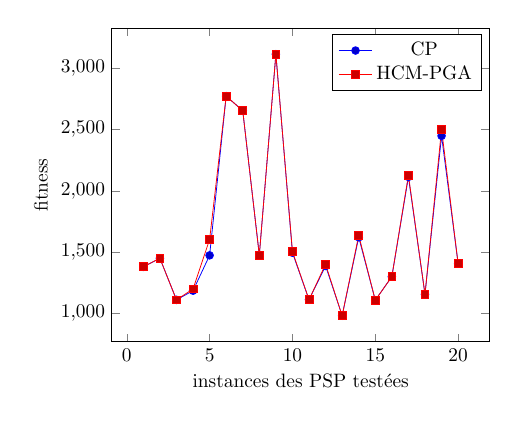
\begin{tikzpicture}[scale=0.7]
       	\begin{axis}[xlabel=instances des PSP testées, ylabel=fitness]
        %\addplot {x^2+2*x-1};
        \addplot coordinates {
        	(1 ,1377)
        	(2 ,1447)
        	(3 ,1107)
        	(4 ,1182)
        	(5 ,1471)
       		(6 ,2774)
       		(7 ,2655)
        	(8 ,1473)
        	(9 ,3117)
        	(10 ,1493)
        	(11 ,1108)
        	(12 ,1384)
        	(13 ,977)
        	(14 ,1619)
        	(15 ,1104)
        	(16 ,1297)
        	(17 ,2113)
        	(18 ,1152)
        	(19 ,2449)
        	(20 ,1403)
        	};
        \addlegendentry{CP}
        \addplot coordinates {
        	(1 ,1378)
        	(2 ,1447)
        	(3 ,1107)
        	(4 ,1196)
        	(5 ,1601)
       		(6 ,2774)
       		(7 ,2655)
        	(8 ,1473)
        	(9 ,3117)
        	(10 ,1502)
        	(11 ,1108)
        	(12 ,1398)
        	(13 ,977)
        	(14 ,1635)
        	(15 ,1104)
        	(16 ,1297)
        	(17 ,2127)
        	(18 ,1152)
        	(19 ,2503)
        	(20 ,1403)
        	};
        \addlegendentry{HCM-PGA}
        \end{axis}
        %\caption{g}
    \end{tikzpicture}
    \end{center}
    \caption{Performances comparées de CP et HCM-PGA en fitness de la meilleure solution trouvée}
    \label{fig:CP_HCM-PGA_best_fitness}
    \end{figure}	
	
	Nous analysons ensuite la performance de HCM-PGA en matière de temps de la meilleure solution trouvée sur nos 10 essais; comme le montre la figure \ref{fig:CP_HCM-PGA_time}, avec pour critère de comparaison le temps de recherche. Nous constatons que le HCM-PGA parcourt bien plus vite l'espace de recherche. Il nous est possible de constater que sur certaines instances le gain de temps est dans le meilleur des cas (instance 10) de 97,21\% . En poursuivant notre analyse, nous pouvons  également faire noter que le temps de recherche est relativement constant. Sur des instances où l'approche CP prend beaucoup plus de temps (instances 6,7,8,9 et 10), notre méthode HCM-PGA conserve un temps de recherche stable. En conséquence, l'usage de notre méthode HCM-PGA s'avère pertinent car elle permet d'avoir sur ces instances, des solutions de bonnes qualités assez rapidement.	
	
	\begin{figure}[!h]
	\begin{center}
	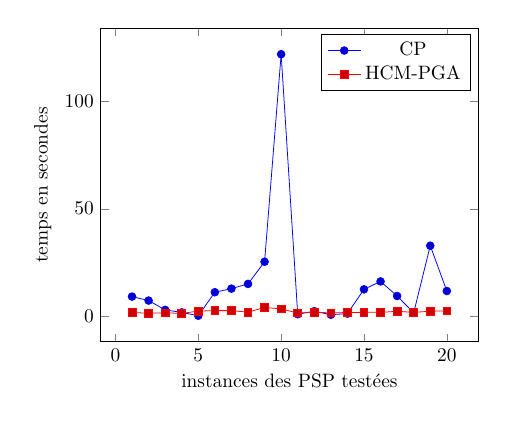
\begin{tikzpicture}[scale=0.7]
       	\begin{axis}[xlabel=instances des PSP testées, ylabel=temps en secondes]
        \addplot coordinates {
        	(1 ,9.14)
        	(2 ,7.29)
        	(3 ,2.94)
        	(4 ,1.78)
        	(5 ,0.23)
       		(6 ,11.17)
       		(7 ,12.84)
        	(8 ,15.03)
        	(9 ,25.35)
        	(10 ,121.90)
        	(11 ,0.935)
        	(12 ,2.347)
        	(13 ,0.711)
        	(14 ,1.223)
        	(15 ,12.508)
        	(16 ,16.187)
        	(17 ,9.404)
        	(18 ,1.589)
        	(19 ,32.811)
        	(20 ,11.726)
        	};
        \addlegendentry{CP}
        \addplot coordinates {
        	(1 ,1.73)
        	(2 ,1.4)
        	(3 ,1.6)
        	(4 ,1.3)
        	(5 ,2.4)
       		(6 ,2.6)
       		(7 ,2.6)
        	(8 ,1.9)
        	(9 ,4.08)
        	(10 ,3.4)
        	(11 ,1.5)
        	(12 ,1.8)
        	(13 ,1.6)
        	(14 ,1.7)
        	(15 ,1.8)
        	(16 ,1.8)
        	(17 ,2.3)
        	(18 ,1.8)
        	(19 ,2.32)
        	(20 ,2.5)
        	};
        \addlegendentry{HCM-PGA}
        \end{axis}
        %\caption{g}
    \end{tikzpicture}
    \caption{Performances comparées de CP et HCM-PGA en temps}
    \label{fig:CP_HCM-PGA_time}
    \end{center}
    \end{figure}
    
    \hspace*{.5cm} En combinant cette analyse ainsi que la précédente, nous pouvons déduire que notre solution HCM-PGA réussit à parcourir l'espace de recherche plus vite que notre approche de référence tout en réussissant sur nos 10 essais tests à trouver une solution optimale ou une solution approchant cette dernière de très près; excepté d'autres instances (instance 5). Nous allons pour la suite, analyser la moyenne des solutions trouvées en matière de performance de fitness.
    
	Trouver une solution proche ou exacte sur un essai est une chose. Arriver à prouver que notre approche trouve des solutions voisines ou proches à la solution exacte sur de nombreux essais est encore une autre chose. La figure \ref{fig:CP_HCM-PGA_moy_fitness} nous permet de dire que notre méthode HCM-PGA peut être efficace dans la résolution des 20 instances présentées et plus largement des instances proposées par Houndji.
    
    \begin{figure}[!h]
    \begin{center}
	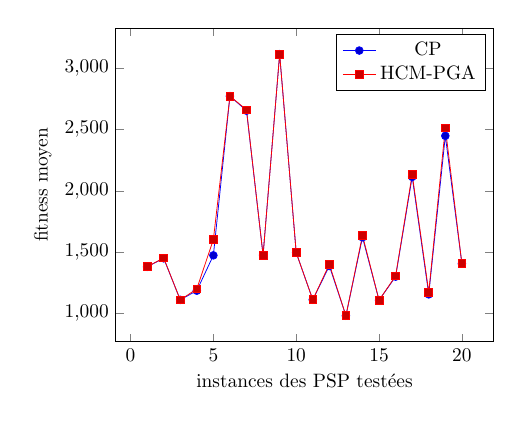
\begin{tikzpicture}[scale=0.7]
       	\begin{axis}[xlabel=instances des PSP testées, ylabel=fitness moyen]
        %\addplot {x^2+2*x-1};
        \addplot coordinates {
        	(1 ,1377)
        	(2 ,1447)
        	(3 ,1107)
        	(4 ,1182)
        	(5 ,1471)
       		(6 ,2774)
       		(7 ,2655)
        	(8 ,1473)
        	(9 ,3117)
        	(10 ,1493)
        	(11 ,1108)
        	(12 ,1384)
        	(13 ,977)
        	(14 ,1619)
        	(15 ,1104)
        	(16 ,1297)
        	(17 ,2113)
        	(18 ,1152)
        	(19 ,2449)
        	(20 ,1403)
        	};
        \addlegendentry{CP}
        \addplot coordinates {
        	(1 ,1378)
        	(2 ,1450)
        	(3 ,1107)
        	(4 ,1196)
        	(5 ,1601)
       		(6 ,2774)
       		(7 ,2662)
        	(8 ,1473)
        	(9 ,3117)
        	(10 ,1493)
        	(11 ,1108)
        	(12 ,1398)
        	(13 ,977)
        	(14 ,1635)
        	(15 ,1104)
        	(16 ,1303)
        	(17 ,2134)
        	(18 ,1171)
        	(19 ,2515)
        	(20 ,1403)
        	};
        \addlegendentry{HCM-PGA}
        \end{axis}
        %\caption{g}
    \end{tikzpicture}
    \end{center}
    \caption{Performances comparées de CP et HCM-PGA en fitness moyen des solutions trouvées}
    \label{fig:CP_HCM-PGA_moy_fitness}
	\end{figure}    
	
    
	\subsection{HFC-PGA et Approche CP}
		Une fois, notre première approche HCM-PGA vérifiée pour les instances proposées par Houndji; nous passons à la seconde méthode de HFC-PGA. La procédure utilisée est similaire à celle utilisée afin de vérifier notre approche HCM-PGA. Nous avons donc analysé les performances en terme de qualité des solutions fournies par notre méthode HFC-PGA. La figure \ref{fig:CP_HFC-PGA_best_fitness} présente les courbes des deux méthodes CP et HFC-PGA. Il en ressort que notre approche HFC-PGA est aussi efficace que l'approche CP. En effet, la déviation maximale sur les 20 instances testées est de  3,2\% (instance 90). Nous estimons cette déviation comme faible. Ainsi, nous pouvons dire que les performances en qualité des meilleures solutions obtenues de l'approche HFC-PGA sont sensiblement égales à celles obtenues de l'approche CP.
    
    \begin{figure}[!h]
    \begin{center}
	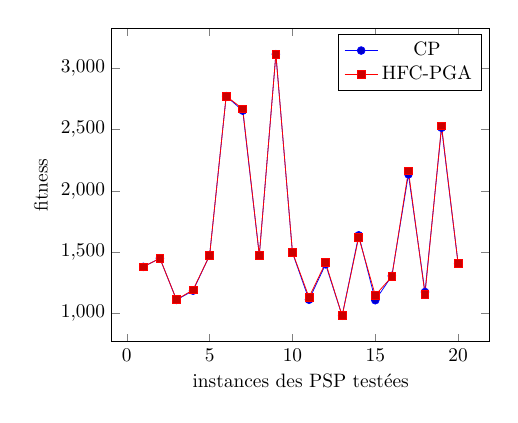
\begin{tikzpicture}[scale=0.7]
       	\begin{axis}[xlabel=instances des PSP testées, ylabel=fitness]
        %\addplot {x^2+2*x-1};
        \addplot coordinates {
        	(1 ,1377)
        	(2 ,1447)
        	(3 ,1107)
        	(4 ,1182)
        	(5 ,1471)
       		(6 ,2774)
       		(7 ,2655)
        	(8 ,1473)
        	(9 ,3117)
        	(10 ,1493)
        	(11 ,1108)
        	(12 ,1398)
        	(13 ,977)
        	(14 ,1635)
        	(15 ,1104)
        	(16 ,1303)
        	(17 ,2134)
        	(18 ,1171)
        	(19 ,2515)
        	(20 ,1403)
        	};
        \addlegendentry{CP}
        \addplot coordinates {
        	(1 ,1377)
        	(2 ,1447)
        	(3 ,1108)
        	(4 ,1189)
        	(5 ,1471)
       		(6 ,2774)
       		(7 ,2670)
        	(8 ,1473)
        	(9 ,3117)
        	(10 ,1497)
        	(11 ,1128)
        	(12 ,1411)
        	(13 ,977)
        	(14 ,1619)
        	(15 ,1145)
        	(16 ,1297)
        	(17 ,2162)
        	(18 ,1152)
        	(19 ,2531)
        	(20 ,1403)
        	};
        \addlegendentry{HFC-PGA}
        \end{axis}
    \end{tikzpicture}
    \end{center}
	\caption{Performances comparées de CP et HFC-PGA en fitness de la meilleure solution trouvée}
	\label{fig:CP_HFC-PGA_best_fitness}
    \end{figure}
    
	La figure \ref{fig:CP_HFC-PGA_time} nous présente les résultats en temps des essais de l'approche HFC-PGA comparés à ceux de l'approche CP. Ainsi, l'approche HFC-PGA parcourt également bien plus vite l'espace de recherche en comparaison à l'approche CP. Un gain de 94,67\% est notamment constaté sur l'instance 10 justifiant la performance en temps de notre solution.    
    
	\begin{figure}[!h]
	
	\begin{center}
	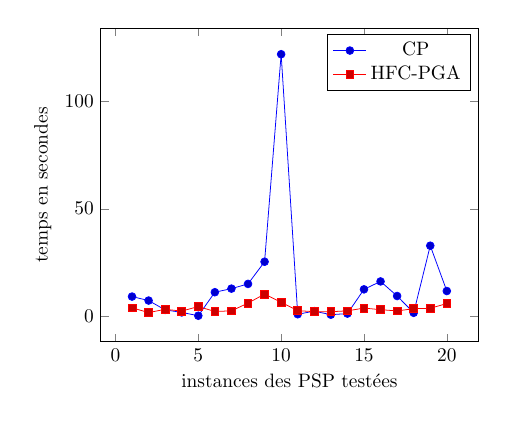
\begin{tikzpicture}[scale=0.7]
       	\begin{axis}[xlabel=instances des PSP testées, ylabel=temps en secondes]
        %\addplot {x^2+2*x-1};
        \addplot coordinates {
        	(1 ,9.14)
        	(2 ,7.29)
        	(3 ,2.94)
        	(4 ,1.78)
        	(5 ,0.23)
       		(6 ,11.17)
       		(7 ,12.84)
        	(8 ,15.03)
        	(9 ,25.35)
        	(10 ,121.90)
        	(11 ,0.935)
        	(12 ,2.347)
        	(13 ,0.711)
        	(14 ,1.223)
        	(15 ,12.508)
        	(16 ,16.187)
        	(17 ,9.404)
        	(18 ,1.589)
        	(19 ,32.811)
        	(20 ,11.726)
        	};
        \addlegendentry{CP}
        \addplot coordinates {
        	(1 ,3.9)
        	(2 ,1.7)
        	(3 ,3.2)
        	(4 ,2.4)
        	(5 ,4.5)
       		(6 ,2.2)
       		(7 ,2.5)
        	(8 ,6.1)
        	(9 ,10.3)
        	(10 ,6.5)
        	(11 ,2.6)
        	(12 ,2.11)
        	(13 ,2.1)
        	(14 ,2.5)
        	(15 ,3.8)
        	(16 ,3.04)
        	(17 ,2.47)
        	(18 ,3.5)
        	(19 ,3.7)
        	(20 ,5.9)
        	};
        \addlegendentry{HFC-PGA}
        \end{axis}
        %\caption{g}
    \end{tikzpicture}
    \end{center}
	\caption{Performances comparées de CP et HFC-PGA en temps}
	\label{fig:CP_HFC-PGA_time}
    \end{figure}
	
	
	Afin de vérifier que notre méthode arrive à trouver en général des solutions proches de la solution optimale, une moyenne de résultats obtenus a été effectuée sur les 10 essais de test. Comme le montre la figure \ref{fig:CP_HFC-PGA_moy_fitness} qui présente les courbes des résultats moyens en terme de qualité du HFC-PGA; nous pouvons remarquer que notre méthode arrive à trouver sur les différents essais effectués des solutions très proches de la solution optimale. En effet, la déviation maximale observée est de 3,3\%. Des observations précédentes et de celle-ci, nous pouvons dire que notre méthode HFC-PGA comme sa seconde HCM-PGA parcourt bien plus vite l'espace de recherche tout en trouvant de solutions optimales sinon très proches de ces dernières.
    \begin{figure}[!h]
    \begin{center}
	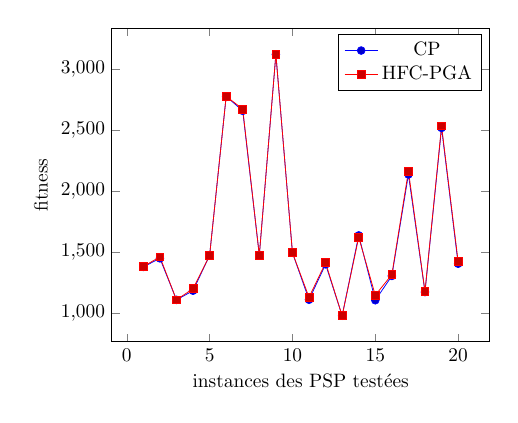
\begin{tikzpicture}[scale=0.7]
       	\begin{axis}[xlabel=instances des PSP testées, ylabel=fitness]
        %\addplot {x^2+2*x-1};
        \addplot coordinates {
        	(1 ,1377)
        	(2 ,1447)
        	(3 ,1107)
        	(4 ,1182)
        	(5 ,1471)
       		(6 ,2774)
       		(7 ,2655)
        	(8 ,1473)
        	(9 ,3117)
        	(10 ,1493)
        	(11 ,1108)
        	(12 ,1398)
        	(13 ,977)
        	(14 ,1635)
        	(15 ,1104)
        	(16 ,1303)
        	(17 ,2134)
        	(18 ,1171)
        	(19 ,2515)
        	(20 ,1403)
        	};
        \addlegendentry{CP}
        \addplot coordinates {
        	(1 ,1380)
        	(2 ,1459)
        	(3 ,1107)
        	(4 ,1199)
        	(5 ,1471)
       		(6 ,2774)
       		(7 ,2670)
        	(8 ,1473)
        	(9 ,3119)
        	(10 ,1493)
        	(11 ,1128)
        	(12 ,1411)
        	(13 ,977)
        	(14 ,1619)
        	(15 ,1145)
        	(16 ,1314)
        	(17 ,2162)
        	(18 ,1177)
        	(19 ,2531)
        	(20 ,1422)
        	};
        \addlegendentry{HFC-PGA}
        \end{axis}
        %\caption{g}
    \end{tikzpicture}
    \end{center}
    \caption{Performances comparées de CP et HFC-PGA en fitness moyen des solutions trouvées}
    \label{fig:CP_HFC-PGA_moy_fitness}
    \end{figure}
    

		\subsection{HCM-PGA et Approche SA}
		
		Les analyses précédentes nous ont permis de dire que nos deux approches basées sur les algorithmes génétiques performent aussi bien en qualité que l'approche CP, tout en parcourant bien plus vite l'espace de recherche. Nous allons dans la suite tenter d'analyser les résultats issus des tests effectués sur des instances bien plus grandes de la bibliothèque Opthub. Ces instances sont en effet plus grandes avec leur horizon de planification supérieur à 200 périodes. La figure \ref{fig:SA_HCM-PGA_time} montre les courbes décrivant l'allure des résultats en temps des deux approches HCM-PGA et SA; et nous permet ainsi de comparer les résultats obtenus. \\
		\hspace*{.5cm} Sur les figures en rapport à l'approche SA, les numéros 1,2,3,4,5 et 6 correspondent respectivement aux instances ps-200-10-80, ps-200-20-80, ps-300-10-80, ps-300-20-80, ps-400-10-80 et ps-400-20-80.
		
		
	\begin{figure}[!h]
    \begin{center}
	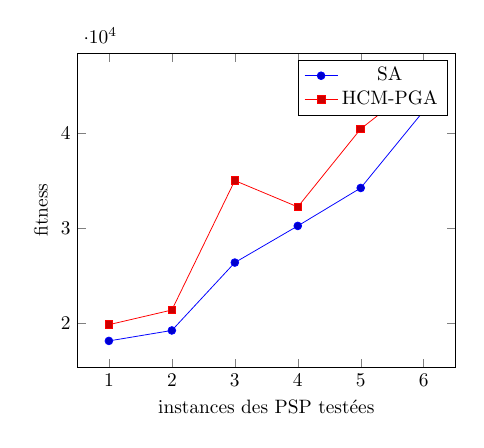
\begin{tikzpicture}[scale=0.7]
       	\begin{axis}[xlabel=instances des PSP testées, ylabel=fitness]
        %\addplot {x^2+2*x-1};
        \addplot coordinates {
        	(1 ,18089)
        	(2 ,19190)
        	(3 ,26343)
        	(4 ,30206)
        	(5 ,34206)
       		(6 ,42329)
        	};
        \addlegendentry{SA}
        \addplot coordinates {
        	(1 ,19799)
        	(2 ,21345)
        	(3 ,34985)
        	(4 ,32207)
        	(5 ,40433)
       		(6 ,45647)
        	};
        \addlegendentry{HCM-PGA}
        \end{axis}
    \end{tikzpicture}
    \end{center}
	\caption{Performances comparées de SA et HCM-PGA en fitness de la meilleure solution trouvée}
	\label{fig:SA_HCM-PGA_best_fitness}
    \end{figure}	
    
	En observant la figure \ref{fig:SA_HCM-PGA_best_fitness}, on constate que les résultats de notre méthode HCM-PGA diffèrent nettement de celles optimales de la méthode SA. On remarque en effet, que la méthode de résolution HCM-PGA trouve des solutions dont le coût est différent de 32\% dans le pire des cas (instance ps-300-10-80). Nous pouvons cependant retenir comme point positif que notre méthode HCM-PGA réussit à approcher de 6.6\% dans le meilleur des cas (instance ps-300-20-80) la solution optimale.
	
	\begin{figure}[!h]
	\begin{center}
	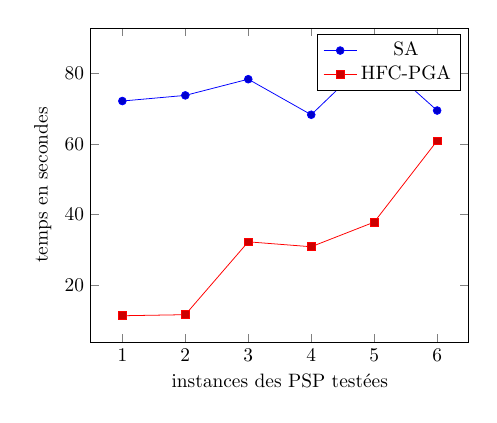
\begin{tikzpicture}[scale=0.7]
       	\begin{axis}[xlabel=instances des PSP testées, ylabel=temps en secondes]
        %\addplot {x^2+2*x-1};
        \addplot coordinates {
        	(1 ,72.2)
        	(2 ,73.8)
        	(3 ,78.4)
        	(4 ,68.3)
        	(5 ,85.5)
       		(6 ,69.5)
        	};
        \addlegendentry{SA}
        \addplot coordinates {
        	(1 ,11.2)
        	(2 ,11.5)
        	(3 ,32.2)
        	(4 ,30.8)
        	(5 ,37.8)
       		(6 ,60.9)
        	};
        \addlegendentry{HFC-PGA}
        \end{axis}
        %\caption{g}
    \end{tikzpicture}
    \end{center}
	\caption{Performances comparées de SA et HCM-PGA en temps}
	\label{fig:SA_HCM-PGA_time}
    \end{figure} 
    
	Notons que notre méthode HCM-PGA ne performe pas aussi bien qu'attendu sur les instances plus grandes lorsqu'on parle de qualité de la meilleure solution trouvée. Nous analysons à présent ses performances en temps. La figure \ref{fig:SA_HCM-PGA_time} nous indique que notre méthode HCM-PGA parcourt toujours aussi vite l'espace de recherche (jusqu'à 84\% de gain en temps dans le meilleur des cas). Nous résumons donc de nos deux analyses en terme de temps et de qualité, que notre méthode HCM-PGA explore toujours aussi vite l'espace de recherche mais ne réussit pas à mieux approcher la solution au delà de 6.6\%.    
    
 
    \subsection{HFC-PGA et Approche SA}	

	La figure \ref{fig:SA_HFC-PGA_best_fitness} présente les résultats des tests effectués en terme de qualité de la solution trouvée. Une analyse similaire à celle menée entre SA et HCM-PGA peut être menée dans le sens où les performances en terme de qualité des solutions obtenues des essais de la méthode HFC-PGA sur les 6 instances plus grandes, ne sont pas aussi intéressantes qu’espérées. En effet, notre méthode de HFC-PGA ne fait pas mieux que 6.4\% dans le meilleur des cas (instance ps-300-20-80). Il est à noter cependant comme point positif que notre méthode HFC-PGA ne fait pas moins bien que 19.2\% de déviation maximale. 
	
	\begin{figure}[!h]
    \begin{center}
	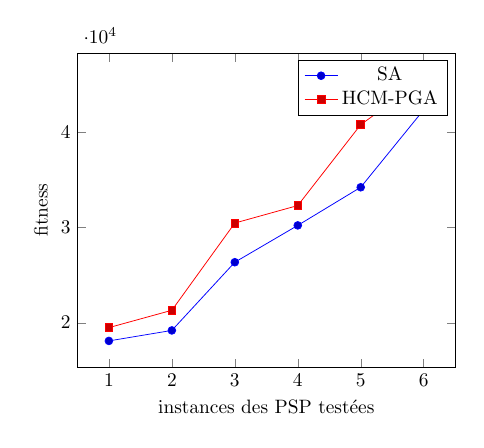
\begin{tikzpicture}[scale=0.7]
       	\begin{axis}[xlabel=instances des PSP testées, ylabel=fitness]
        %\addplot {x^2+2*x-1};
        \addplot coordinates {
        	(1 ,18089)
        	(2 ,19190)
        	(3 ,26343)
        	(4 ,30206)
        	(5 ,34206)
       		(6 ,42329)
        	};
        \addlegendentry{SA}
        \addplot coordinates {
        	(1 ,19484)
        	(2 ,21302)
        	(3 ,30452)
        	(4 ,32289)
        	(5 ,40775)
       		(6 ,45521)
        	};
        \addlegendentry{HCM-PGA}
        \end{axis}
    \end{tikzpicture}
    \end{center}
	\caption{Performances comparées de SA et HFC-PGA en fitness de la meilleure solution trouvée}
	\label{fig:SA_HFC-PGA_best_fitness}
    \end{figure} 	
	
	Du point de vue de la performance en temps de notre méthode comparée à la méthode SA, plus l'horizon de planification s'étend plus, l'efficacité en temps se dégrade. En effet, elle est de 9.9 secondes sur un horizon de 200 périodes et de 120 secondes sur un horizon de 400 périodes; environ deux fois plus que le temps pris par la méthode SA pour cette dernière instance comme le montre la figure \ref{fig:SA_HFC-PGA_time}.
	\begin{figure}[!h]
	\begin{center}
	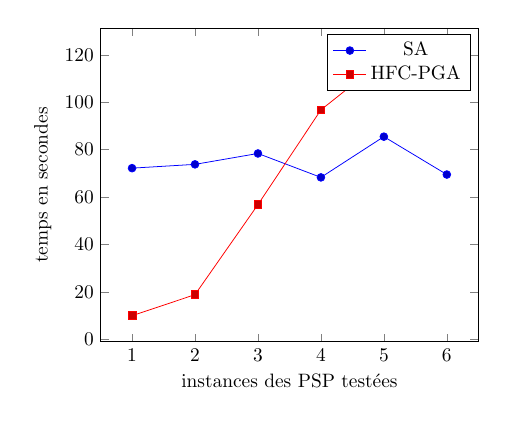
\begin{tikzpicture}[scale=0.7]
       	\begin{axis}[xlabel=instances des PSP testées, ylabel=temps en secondes]
        %\addplot {x^2+2*x-1};
        \addplot coordinates {
        	(1 ,72.2)
        	(2 ,73.8)
        	(3 ,78.4)
        	(4 ,68.3)
        	(5 ,85.5)
       		(6 ,69.5)
        	};
        \addlegendentry{SA}
        \addplot coordinates {
        	(1 ,9.9)
        	(2 ,18.8)
        	(3 ,56.8)
        	(4 ,96.8)
        	(5 ,117.9)
       		(6 ,120.3)
        	};
        \addlegendentry{HFC-PGA}
        \end{axis}
        %\caption{g}
    \end{tikzpicture}
    \end{center}
	\caption{Performances comparées de SA et HFC-PGA en temps}
	\label{fig:SA_HFC-PGA_time}
    \end{figure}
        	
    
		\subsection{HCM-PGA et HFC-PGA}

	Dans cette section, nous tentons de répondre à la question de savoir laquelle des méthodes HCM-PGA et HFC-PGA est la plus pertinente dans la résolution des problèmes du PSP en nous basant sur les résultats des tests effectués sur les instances proposées par Houndji. Les figures \ref{fig:HCM-PGA_HFC-PGA_time} et \ref{fig:HCM-PGA_HFC-PGA_moy_fitness} présentent respectivement les résultats en terme de temps et de qualité. On note ainsi globalement que la méthode de HCM-PGA est plus rapide que celle du HFC-PGA et également plus précise que cette dernière lorsqu’on parle de qualité des solutions trouvées. Nous nous expliquons cela sans doute par le fait que les algorithmes génétiques parallèles et hiérarchiques HFC-PGA doivent faire démarrer un grand nombre de nœuds (ou threads) correspondants chacune à un chromosome afin de pouvoir explorer l'espace de recherche ainsi qu'à la topologie utilisée dans le HFC-PGA.
		
		
	\begin{figure}[!h]
	\begin{center}
	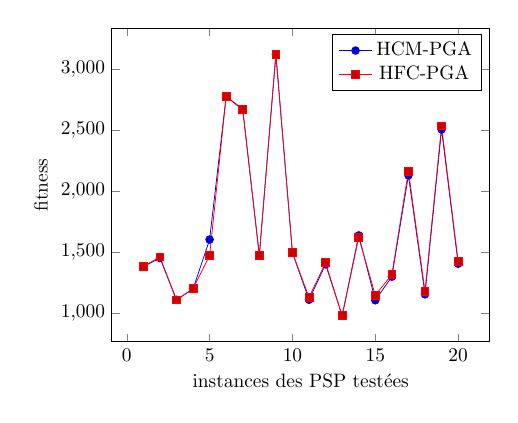
\begin{tikzpicture}[scale=0.7]
       	\begin{axis}[xlabel=instances des PSP testées, ylabel=fitness]
        %\addplot {x^2+2*x-1};
        \addplot coordinates {
        	(1 ,1378)
        	(2 ,1450)
        	(3 ,1107)
        	(4 ,1196)
        	(5 ,1601)
       		(6 ,2774)
       		(7 ,2662)
        	(8 ,1473)
        	(9 ,3117)
        	(10 ,1493)
        	(11 ,1108)
        	(12 ,1398)
        	(13 ,977)
        	(14 ,1635)
        	(15 ,1104)
        	(16 ,1297)
        	(17 ,2127)
        	(18 ,1152)
        	(19 ,2503)
        	(20 ,1403)
        	};
        \addlegendentry{HCM-PGA}
        \addplot coordinates {
        	(1 ,1380)
        	(2 ,1459)
        	(3 ,1107)
        	(4 ,1199)
        	(5 ,1471)
       		(6 ,2774)
       		(7 ,2670)
        	(8 ,1473)
        	(9 ,3119)
        	(10 ,1493)
        	(11 ,1128)
        	(12 ,1411)
        	(13 ,977)
        	(14 ,1619)
        	(15 ,1145)
        	(16 ,1314)
        	(17 ,2162)
        	(18 ,1177)
        	(19 ,2531)
        	(20 ,1422)
        	};
        \addlegendentry{HFC-PGA}
        \end{axis}
        %\caption{g}
    \end{tikzpicture}
    \end{center}
    \caption{Performances comparées de HCM-PGA et HFC-PGA en fitness moyen des solutions trouvées}
    \label{fig:HCM-PGA_HFC-PGA_moy_fitness}
    \end{figure}
    
    \begin{figure}[!h]
	
	\begin{center}
	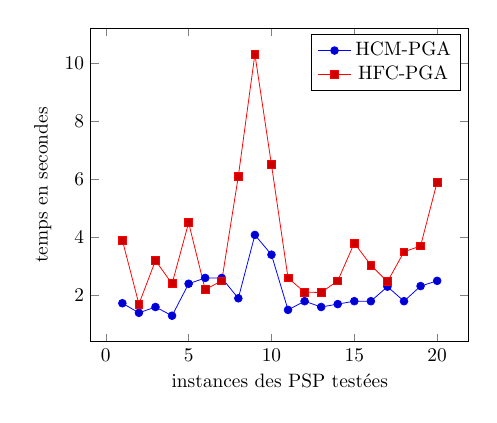
\begin{tikzpicture}[scale=0.7]
       	\begin{axis}[xlabel=instances des PSP testées, ylabel=temps en secondes]
        %\addplot {x^2+2*x-1};
        \addplot coordinates {
        	(1 ,1.73)
        	(2 ,1.4)
        	(3 ,1.6)
        	(4 ,1.3)
        	(5 ,2.4)
       		(6 ,2.6)
       		(7 ,2.6)
        	(8 ,1.9)
        	(9 ,4.08)
        	(10 ,3.4)
        	(11 ,1.5)
        	(12 ,1.8)
        	(13 ,1.6)
        	(14 ,1.7)
        	(15 ,1.8)
        	(16 ,1.8)
        	(17 ,2.3)
        	(18 ,1.8)
        	(19 ,2.32)
        	(20 ,2.5)
        	};
        \addlegendentry{HCM-PGA}
        \addplot coordinates {
        	(1 ,3.9)
        	(2 ,1.7)
        	(3 ,3.2)
        	(4 ,2.4)
        	(5 ,4.5)
       		(6 ,2.2)
       		(7 ,2.5)
        	(8 ,6.1)
        	(9 ,10.3)
        	(10 ,6.5)
        	(11 ,2.6)
        	(12 ,2.11)
        	(13 ,2.1)
        	(14 ,2.5)
        	(15 ,3.8)
        	(16 ,3.04)
        	(17 ,2.47)
        	(18 ,3.5)
        	(19 ,3.7)
        	(20 ,5.9)
        	};
        \addlegendentry{HFC-PGA}
        \end{axis}
    \end{tikzpicture}
    \end{center}
    
	\caption{Performances comparées de HCM-PGA et HFC-PGA en temps}
	\label{fig:HCM-PGA_HFC-PGA_time}
    \end{figure} 
    
		\section*{Conclusion}
		\addcontentsline{toc}{section}{Conclusion}
		Les tests effectués dans cette partie ont été l'occasion de vérifier nos deux méthodes de résolution proposées basées sur les algorithmes génétiques. Nous avons ainsi pu comparer chacune d'elles aux approches CP et SA et avons pu tirer des conclusions. Il ne nous reste plus qu'à conclure notre étude et à présenter les perspectives envisagées.